% Convolution operator.
% Author: Janosh Riebesell
% Adapted from https://tikz.net/conv2d/, which is in turn
% Adapted from https://github.com/PetarV-/TikZ/tree/master/2D%20Convolution

\documentclass[tikz]{standalone}

\usetikzlibrary{matrix, positioning}

\definecolor{orblue}{RGB}{0, 90, 169} 
\definecolor{logred}{RGB}{185, 15, 34}
\definecolor{tugreen}{RGB}{127, 171, 22}

\begin{document}
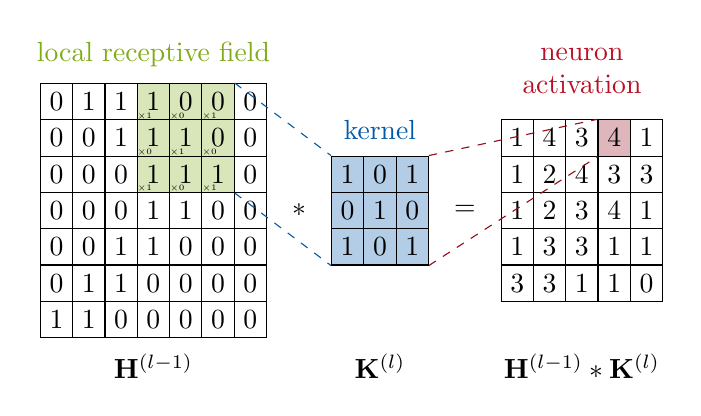
\begin{tikzpicture}[
    2d-arr/.style={matrix of nodes, row sep=-\pgflinewidth, column sep=-\pgflinewidth, nodes={draw}}
  ]

  \matrix (mtr) [2d-arr] {
  0 & 1 & 1 & |[fill=tugreen!30]| 1 & |[fill=tugreen!30]| 0 & |[fill=tugreen!30]| 0 & 0\\
  0 & 0 & 1 & |[fill=tugreen!30]| 1 & |[fill=tugreen!30]| 1 & |[fill=tugreen!30]| 0 & 0\\
  0 & 0 & 0 & |[fill=tugreen!30]| 1 & |[fill=tugreen!30]| 1 & |[fill=tugreen!30]| 1 & 0\\
  0 & 0 & 0 & 1 & 1 & 0 & 0\\
  0 & 0 & 1 & 1 & 0 & 0 & 0\\
  0 & 1 & 1 & 0 & 0 & 0 & 0\\
  1 & 1 & 0 & 0 & 0 & 0 & 0\\
  };

  \node[below=of mtr-5-4] {$\mathbf{H}^{(l-1)}$};

  \node[right=0.2em of mtr] (str) {$*$};

  \matrix (K) [2d-arr, right=0.2em of str, nodes={draw, fill=orblue!30}] {
    1 & 0 & 1 \\
    0 & 1 & 0 \\
    1 & 0 & 1 \\
  };
  \node[below=of K-3-2] {$\mathbf{K}^{(l)}$};

  \node[right=0.2em of K] (eq) {$=$};

  \matrix (ret) [2d-arr, right=0.2em of eq] {
  1 & 4 & 3 & |[fill=logred!80!black!30]| 4 & 1\\
  1 & 2 & 4 & 3 & 3\\
  1 & 2 & 3 & 4 & 1\\
  1 & 3 & 3 & 1 & 1\\
  3 & 3 & 1 & 1 & 0\\
  };
  \node[below=of ret-4-3] {$\mathbf{H}^{(l-1)} * \mathbf{K}^{(l)}$};
  \node[above=of ret-3-3] {\textcolor{logred}{\begin{tabular}{c} neuron \\ activation \end{tabular}}};
  \node[above=of K-3-2] {\textcolor{orblue}{kernel}};
  \node[above=of mtr-3-4] {\textcolor{tugreen}{local receptive field}};

  \draw[dashed, orblue] (mtr-1-6.north east) -- (K-1-1.north west);
  \draw[dashed, orblue] (mtr-3-6.south east) -- (K-3-1.south west);

  \draw[dashed, logred!80!black] (K-1-3.north east) -- (ret-1-4.north west);
  \draw[dashed, logred!80!black] (K-3-3.south east) -- (ret-1-4.south west);

  \foreach \i in {1,2,3} {
      \foreach \j in {4,5,6} {
          \node[font=\tiny, scale=0.6, shift={(-1.2ex,-2ex)}] at (mtr-\i-\j) {$\times \pgfmathparse{int(mod(\i+\j,2))}\pgfmathresult$};
        }
    }

\end{tikzpicture}
\end{document}